\documentclass[11pt,a4paper]{article}
\usepackage{amsmath}
\usepackage{amsfonts}
\usepackage{amssymb}
\usepackage{fancyhdr}
\usepackage{lastpage}
\usepackage{graphicx}
\usepackage{ucs}
\usepackage[utf8x]{inputenc}
\usepackage[italian]{babel}

\renewcommand{\headrulewidth}{0.6pt}
\renewcommand{\footrulewidth}{0.6pt}
% impostazione dello stile per le pagine interne del documento
\lhead{\leftmark}
\chead{}
\rhead{
\includegraphics[scale=0.15]{logo.png} }
\lfoot{Analisi dei requisiti v0.7.3}
\cfoot{}
\rfoot{\thepage \ di \pageref{LastPage}}
% ridefinizione dello stile plain per il frontespizio
\fancypagestyle{plain}{
\fancyhf
}
% impostazione dello stile per l'indice
\fancypagestyle{indice}{
\lhead{\leftmark}
\chead{}
\rhead{
\includegraphics[scale=0.15]{logo.png}}
\lfoot{Analisi dei requisiti v0.7.3}
\cfoot{}
\rfoot{}
}
\headheight = 46pt
%definizione del comando "\modifiche" per la creazione del diario delle modifiche
\newcommand{\modifiche} 
{
\newpage
\begin{center}
\textbf{Diario delle modifiche} \\
\bigskip
\begin{tabular}{|c|c|p{0.51\textwidth}|}
\hline
\textsc{Data} & \textsc{Versione} & \textsc{Modifica} \\
\hline
\hline
\textit{7 dicembre 2008} & 0.7.3 & Correzione di errori di forma e sintassi\\
\hline
\textit{6 dicembre 2008} & 0.7.2 & Correzione degli use case \\
\hline
\textit{4 dicembre 2008} & 0.7.1 & Selezione dei termini contenuti nel glossario \\
\hline
\textit{4 dicembre 2008} & 0.7.0 & Stesura del sommario \\
\hline
\textit{2 dicembre 2008} & 0.6.0 & Completamento stesura della descrizione del prodotto \\
\hline
\textit{2 dicembre 2008} & 0.5.0 & Stesura degli use case \\
\hline
\textit{1 dicembre 2008} & 0.4.1 & Correzione dei requisiti \\
\hline
\textit{30 novembre 2008} & 0.4.0 & Stesura dei requisiti \\
\hline
\textit{29 novembre 2008} & 0.3.0 & Inizio stesura della descrizione del prodotto \\
\hline
\textit{28 novembre 2008} & 0.2.0 & Stesura dell'introduzione \\
\hline
\textit{28 novembre 2008} & 0.1.0 & Stesura dell'indice \\
\hline
\end{tabular}
\end{center}
}
%definizione del comando "\info" per la creazione delle informazioni del documento
\newcommand{\info} {
\bigskip
\begin{tabbing}
	\hspace*{0.3\textwidth} \= \hspace*{0.5\textwidth} \kill
	\parbox{0.3\textwidth}{\textbf{Verifica: }} \> \parbox{0.5\textwidth}{Freo Matteo} \\
	\parbox{0.3\textwidth}{\textbf{Approvazione: }} \> \parbox{0.5\textwidth}{Scortegagna Carlo} \\
	\parbox{0.3\textwidth}{\textbf{Stato: }} \> \parbox{0.5\textwidth}{Formale} \\
	\parbox{0.3\textwidth}{\textbf{Uso: }} \> \parbox{0.5\textwidth}{Esterno} \\
	\parbox{0.3\textwidth}{\textbf{Distribuzione: }} \> \parbox{0.5\textwidth}{QuiXoft} \\
							\> \parbox{0.5\textwidth}{Rossi Francesca} \\
							\> \parbox{0.5\textwidth}{Vardanega Tullio} \\
							\> \parbox{0.5\textwidth}{Conte Renato} \\
\end{tabbing}
}
%definizione del comando "\frontespizio" per la creazione del frontespizio
\newcommand{\frontespizio} {
\thispagestyle{plain}
\title{\begin{Huge}\textsc{Progetto SIGEOL}\end{Huge} \\ \textit{Analisi dei requisiti \\ v0.7.3}}
\author{Redazione: Beggiato Andrea, Scarpa Davide, Barbiero Mattia }
\maketitle
\medskip
\begin{center}

\includegraphics[scale=0.5]{logo.png} \\
\textit{quixoft.sol@gmail.com}
\end{center}
\medskip
\info
\begin{center}
\textbf{Sommario} \\
Documento contenente l'analisi dei requisiti per il progetto ``SIGEOL'' commissionato dalla prof. Rossi Francesca.
\end{center}
\newpage
}
%definizione del comando "\indice" per la creazione dell'indice
\newcommand{\indice} {
\thispagestyle{indice}
\tableofcontents
\newpage
}
\pagestyle{fancy}
\begin{document}
\frontespizio
\indice
\setcounter{page}{1}
\section{Introduzione}
\subsection{Scopo del documento}
Il presente documento denominato \textsc{Analisi dei requisiti} ha lo scopo di delineare tutti i bisogni espressi dal committente Prof. Rossi Francesca per il sistema ``SIGEOL'', nonchè tutti i requisiti intrinsechi nello sviluppo di un tale prodotto.

Nel caso in cui la proposta venga ritenuta adeguata il seguente documento avrà valenza contrattuale e concretizzerà un legame di reciproco interesse tra il team QuiXoft ed il cliente al quale il documento è rivolto.
\subsection{Scopo del prodotto}
Il progetto sotto analisi, denominato \textit{SIGEOL}, si prefigge di automatizzare la generazione, la gestione, l'ottimizzazione e la consultazione degli orari di lezione. Il committente richiede l'applicazione del sistema al solo corso di laurea in Informatica, ma, constatato che la complessità non aumenta notevolmente, il team QuiXoft prevede lo sviluppo e la messa in opera dell'applicazione per tutti i corsi di laurea dell' Università degli studi di Padova.

Il prodotto sarà implementato come un \underline{servizio web} \underline{portabile}, facilmente manutenibile ed \underline{accessibile} agli utenti da una qualsiasi postazione con accesso alla rete Internet.
\subsection{Glossario}
Le definizioni dei termini specialistici usati nella stesura di questo e di tutti gli altri documenti possono essere trovate nel documento \textsc{Glossario} al fine di eliminare ogni ambiguità e di facilitare la comprensione dei temi trattati. Ogni termine la cui definizione è disponibile all’interno del Glossario verrà marcato con una \underline{sottolineatura}.
\subsection{Riferimenti}
\begin{itemize}
 \item Capitolato d'appalto reperibile all'indirizzo: \\ http://www.math.unipd.it/~tullio/IS-1/2008/Progetti/SIGEOL.html
 \item Statuto di Ateneo reperibile all'indirizzo \\ http://www.unipd.it/organizzazione/statuto/statuto.htm
 \item Informativa sulla privacy (Legge per il trattamento dei dati personali)
 \item Incontri con il committente
\end{itemize}

\section{Descrizione generale}
\subsection{Contesto d'uso del prodotto}
\subsubsection{Processi produttivi e modalità d'uso}
Il funzionamento del sistema \textit{SIGEOL}, a processo produttivo concluso, sarà in grado di guidare ogni singolo utilizzatore (confronta sezione \ref{utenti}) allo svolgimento delle proprie azioni (confronta sezione \ref{funzioni}). In altre parole sarà disponibile un servizio che offrirà, dopo un'opportuna \underline{autenticazione}, un insieme di strumenti che permetteranno l'inserimento guidato dei dati che serviranno al fine ultimo di generare un orario per le lezioni.
\subsubsection{Piattaforma d’esecuzione ed interfacciamento con l’ambiente di installazione e uso}
Il prodotto sarà realizzato tramite un'applicazione web supportata da un \underline{database} e dovrà essere accessibile da un qualsiasi tipo di \underline{browser}. Data la mancanza di un applicativo preesistente al quale aggiungere le funzioni del sistema \textit{SIGEOL}, il team QuiXoft dovrà definirne ogni aspetto creando un prodotto che sia \underline{accessibile}, manutenibile, \underline{portabile} e soprattutto sicuro. A tal scopo verranno adottate tecnologie gratuite e moderne per lo sviluppo di pagine dinamiche e sarà necessario disporre di un \underline{server} affidabile.
\subsection{Funzioni del prodotto} \label{funzioni}
Il prodotto consentirà, alle varie tipoligie di utenti, di fruire di un servizio che permetta la generazione e l'ottimizzazione di uno schema d'orario per le lezioni. Per raggiungere questo scopo i vari utenti dovranno inserire i dati di loro competenza richiesti dal sistema, tra i quali figurano vincoli e preferenze.

L'applicazione dovrà soddisfare necessariamente i vincoli nel loro insieme, senza tralasciarne alcuno, mentre, per quanto riguarda il soddisfacimento delle preferenze, il sistema cercherà di tenerne conto il più possibile, restando consapevole di poterne tralasciare.

Nel caso risulti impossibile soddisfare tutti i vincoli, il prodotto segnalerà una soluzione per raggiungere lo scopo della generazione dell'orario.

Per informazioni più dettagliate confrontare la sezione \ref{requisiti}
\subsection{Caratteristiche degli utenti} \label{utenti}
Si prevedono cinque tipologie di utenti che usufruiranno del sistema:
\begin{itemize}
 \item Segreteria generale
 \item Segreteria didattica
 \item Presidente del CCS
 \item Docente
 \item Utente non autenticato
\end{itemize}

La \textit{segreteria generale} si occupa dell'invito delle varie \textit{segreterie didattiche}, nonchè della preparazione della struttura delle varie facoltà.

La \textit{segreteria didattica} ha, tra gli altri, il compito di invitare i \textit{presidenti del CCS} dei vari corsi di laurea e di inserire i corsi della facoltà di sua competenza.

Il \textit{presidente del CCS} provvede, invece, all'invito dei vari \textit{docenti} che dovranno compilare i propri dati ed accettare il consenso al loro trattamento.

L' \textit{utente non autenticato} sarà in grado di consultare le informazioni che verranno rese disponibili dal sistema, quali schemi d'orario, informazioni su docenti, aule, corsi di laurea e corsi.

Ogni tipologia potrà inserire i propri vincoli e preferenze (esclusi gli utenti non autenticati) e, dato che il sistema ``SIGEOL'' guiderà nel modo più accurato possibile ogni utente, non sono richieste particolari conoscescenze ad eccezione dell'uso di un elaboratore connesso alla rete Internet.
\subsection{Vincoli generali}
Il sistema che si intende sviluppare cercherà di essere il più \underline{portabile} ed indipendente possibile. Il team QuiXoft non esclude però che sia necessaria l'installazione di componenti software nel \underline{server} dove il prodotto risiederà. Ad ogni modo non saranno in alcun modo utilizzate tecnologie soggette al pagamento di una qualche forma di licenza o altro.
\subsection{Assunzioni e dipendenze}
Il prodotto che il team QuiXoft si impegna a sviluppare dipende da diversi fattori quali:
\begin{itemize}
 \item Documentazione fornita dal committente
 \item Disponibilità del committente ad incontri e chiarimenti richiesti dal team.
\end{itemize}
Inoltre il team QuiXoft si rende consapevole della possibilità di cambiamento od aggiunta di aluni requisiti da parte del committente in corso d'opera.
\section{Requisiti} \label{requisiti}
In questa sezione verranno elencati i requisiti del prodotto, organizzati per tipologia di utente per facilitarne la lettura. Sarà inoltre utilizzata una distinzione tra requisiti obbligatori, desiderabili ed opzionali.
\subsection{Requisiti funzionali}
\subsubsection{Requisiti funzionali per la segreteria generale}
\begin{itemize}
\item \textbf{OBBLIGATORI}
\begin{enumerate}
\item Possibilità di \underline{autenticazione}
\item Possibilità di inserimento delle facoltà
\item Possibilità di invitare via e-mail le singole facoltà ad inserire i dati
\item Possibilità di consultare lo schema d'orario di ogni corso di laurea
\end{enumerate}
\item \textbf{DESIDERABILI}
\begin{enumerate}
\item Possibilità di impostare la frequenza con cui avviene il \underline{backup} automatico dei dati
\item Possibilità di ripristinare i dati relativi alle facoltà da un \underline{backup} scelto
\item Possibilità di consultare le informazioni relative a docenti, aule, corsi di laurea e corsi.
\end{enumerate}
\end{itemize}
\subsubsection{Requisiti funzionali per la segreteria didattica}
\begin{itemize}
\item \textbf{OBBLIGATORI}
\begin{enumerate}
\item Possibilità di \underline{autenticazione}
\item Possibilità di inserimento e modifica per ogni corso, all'interno della propria facoltà, del nome, dei relativi CFU, dell'anno di appartenenza, del periodo, dello stato, del numero di ore in aula e in laboratorio (se previsto), del docente di riferimento che lo tiene, di eventuali assistenti e della stima del numero di studenti che lo seguiranno
\item Possibilità di inserimento e modifica per ogni aula disponibile, all'interno della propria facoltà, del nome, della capienza, delle ore e dei periodi di non disponibilità
\item Possibilità di inserimento e modifica dell'anno accademico
\item Possibilità di impostare vincoli e preferenze per ogni corso di laurea
\item Possibilità di modifica dei dati dei docenti preventivamente inseriti dal Presidente del CCS
\item Possibilità di invitare via e-mail i presidenti del CCS di ogni corso di laurea ad inserire i dati
\item Possibilità di ripristinare i dati relativi ai corsi di laurea da un \underline{backup} scelto
\end{enumerate}
\item \textsc{DESIDERABILI}
\begin{enumerate}
\item Possibilità di generazione dello schema d'orario in formato \underline{pdf} e \underline{html}
\item Possibilità di scegliere vincoli da rilassare proposti dal sistema in caso di soluzione inesistente
\item Possibilità di consultare lo schema d'orario di ogni corso di laurea
\item Possibilità di consultare le informazioni relative a docenti, aule, corsi di laurea e corsi
\end{enumerate}
\end{itemize}
\subsubsection{Requisiti funzionali per il Presidente del CCS}
\begin{itemize}
\item \textbf{OBBLIGATORI}
\begin{enumerate}
\item Possibilità di \underline{autenticazione}
\item Possibilità di inserimento e modifica per ogni corso, all'interno del proprio corso di laurea, del nome, dei relativi CFU, dell'anno di appartenenza, del periodo, dello stato, del numero di ore in aula e in laboratorio (se previsto), del docente di riferimento che lo tiene, di eventuali assistenti e della stima del numero di studenti che lo seguiranno
\item Possibilità di inserimento e modifica per ogni aula disponibile, all'interno del proprio corso di laurea, del nome, della capienza, delle ore e dei periodi di non disponibilità
\item Possibilità di inserimento e modifica, all'interno del proprio corso di laurea, dei dati dei docenti
\item Possibilità di inserimento e modifica dell'anno accademico
\item Possibilità di impostare vincoli e preferenze per ogni corso
\item Possibilità di generazione dello schema d'orario in formato \underline{pdf} e \underline{html}
\item Possibilità di scegliere vincoli da rilassare proposti dal sistema in caso di soluzione inesistente
\item Possibilità di consultare lo schema d'orario
\item Possibilità di inserimento e modifica di indirizzi diversi appartenenti allo stesso corso di laurea
\item Possibilità di ripristinare i dati relativi ai corsi da un \underline{backup} scelto
\item Possibilità di notificare i docenti nel caso di vincoli e preferenze non soddisfatti
\end{enumerate}
\item \textbf{DESIDERABILI}
\begin{enumerate}
\item Possibilità di notificare il mancato inserimento di un docente o di un corso d'insegnamento di un altro corso di laurea
\item Possibilità di impostare una data limite per l'inserimento dei vincoli da parte dei docenti, con notifica della scadenza.
\item Possibilità di modifica manuale dello schema d'orario specificato
\item Possibilità di consultare le informazioni relative a docenti, aule, corsi di laurea e corsi
\end{enumerate}
\end{itemize}
\subsubsection{Requisiti funzionali per i docenti}
\begin{itemize}
\item \textsc{OBBLIGATORI}
\begin{enumerate}
\item Possibilità di inserimento e modifica dei propri giorni e ore di indisponibilità, con relativa motivazione
\item Possibilità di inserimento e modifica delle proprie preferenze su orari e giorni di lezione, con relativa motivazione
\item Possibilità di modifica dei propri dati personali
\end{enumerate}
\item \textbf{DESIDERABILI}
\begin{enumerate}
\item Possibilità di consultare le informazioni relative a docenti, aule, corsi di laurea e corsi
\end{enumerate}
\end{itemize}
\subsubsection{Requisiti funzionali per l'Utente non autenticato}
\begin{itemize}
\item \textbf{DESIDERABILI}
\begin{enumerate}
\item Possibilità di consultare lo schema d'orario
\item Possibilità di consultare le informazioni relative a docenti, aule, corsi di laurea e corsi
\end{enumerate}
\end{itemize}
\subsection{Requisiti di qualità}
\begin{itemize}
\item \textbf{OBBLIGATORI}
\begin{enumerate}
\item \underline{Accessibilità} del sistema
\item Garanzie sull'integrità dei dati
\item Gestione in sicurezza degli \underline{account}
\item Manutenibilità del sistema
\item Interfaccia utente semplice e intuitiva
\item Presenza di manuali d'uso, di installazione, configurazione e manutenzione del sistema
\item Il prodotto dovrà essere consegnato assieme ad un \underline{ambiente di prova} per verificarne il corretto funzionamento
\end{enumerate}
\item \textbf{DESIDERABILI}
\begin{enumerate}
\item Portabilità del sistema
\item Completa interoperabilità dei dati memorizzati e trattati
\item Pagine scritte in \underline{XHTML} e \underline{CCS} dovranno essere validate tramite strumenti forniti dal consorzio \underline{W3C}
\end{enumerate}
\end{itemize}
\subsection{Requisiti d'interfacciamento e d'ambiente}
\subsubsection{Con l’ambiente di installazione ed uso}
\begin{itemize}
\item \textbf{OBBLIGATORI}
\begin{enumerate}
\item Le informazioni andranno memorizzate in modo permanente in un \underline{database}
\end{enumerate}
\item \textbf{DESIDERABILI}
\begin{enumerate}
\item Le tecnologie da adottare dovranno essere gratuite
\end{enumerate}
\end{itemize}
\subsubsection{Con l’operatore}
\begin{itemize}
\item \textbf{OBBLIGATORI}
\begin{enumerate}
\item Le informazioni dovranno essere acquisite tramite un \underline{servizio web}
\item Il sistema distinguerà i vari tipi di utente tramite \underline{autenticazione}
\item Al fine di evitare errori il sistema dovrà il più possibile proporre all'utente i dati in modo automatico
\end{enumerate}
\end{itemize}
\section{Use case e descrizioni narrative}
In questo capitolo verranno illustrati i \underline{diagrammi use-case} che rappresentano
i requisiti funzionali del prodotto.

I diagrammi verrano accompagnati dalle loro descrizioni narrative per consentirne
una migliore comprensione.
\subsection{Use case generale}
Il seguente diagramma illustra in modo generale le funzionalità offerte dal sistema ``SIGEOL'' .
\begin{center}
 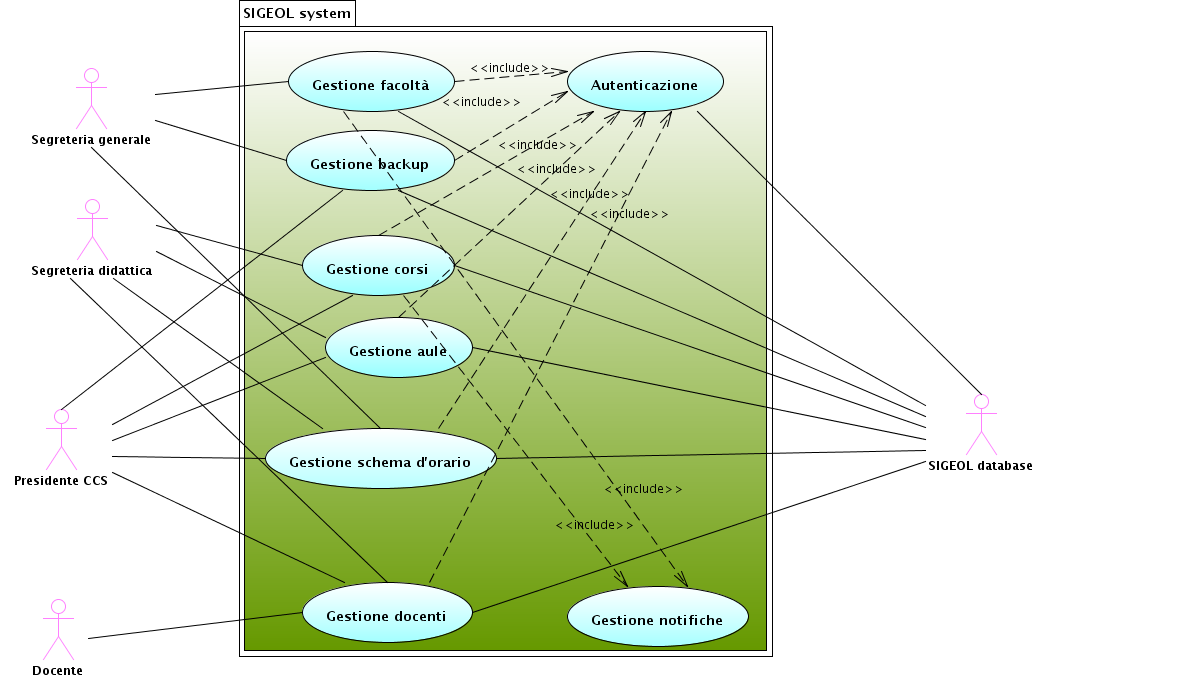
\includegraphics[scale=0.5]{UseCaseSistema.png}
 % UseCaseSistema.png: 638x495 pixel, 72dpi, 22.51x17.46 cm, bb=0 0 638 495
\end{center}

Il sistema è composto da dieci parti principali:
\begin{enumerate}
\item Gestione facoltà: modulo per la gestione dei dati relativi alle facoltà. 
\item Gestione corsi di laurea: modulo per la gestione dei dati relativi ai corsi di laurea.
\item Gestione corsi: modulo per la gestione dei dati relativi ai corsi di lezione.
\item Gestione aule: modulo per la gestione dei dati relativi alle aule.
\item Gestione docenti: modulo per la gestione dei dati relativi ai docenti.
\item Gestione schema d'orario: modulo per la gestione e la generazione dello schema d'orario.
\item Gestione backup: modulo per la gestione dei \underline{backup} del SIGEOL \underline{database}.
\item Autenticazione: modulo utilizzato per \underline{autenticare} le varie tipologie di utenti.
\item Gestione notifiche: modulo per la gestione delle notifiche.
\item Gestione consultazione: modulo per la visualizzazione delle informazione relative ai corsi di laurea, corsi di lezione, docenti, aule e schema d'orario
\end{enumerate}
\textbf{Attori coinvolti:}
\textit{segreteria generale}, \textit{segreteria didattica}, \textit{presidente CCS}, \textit{docente}, \textit{utente non autenticato}, \textit{SIGEOL \underline{database}}
\subsection{Use case Autenticazione}
\begin{center} 
 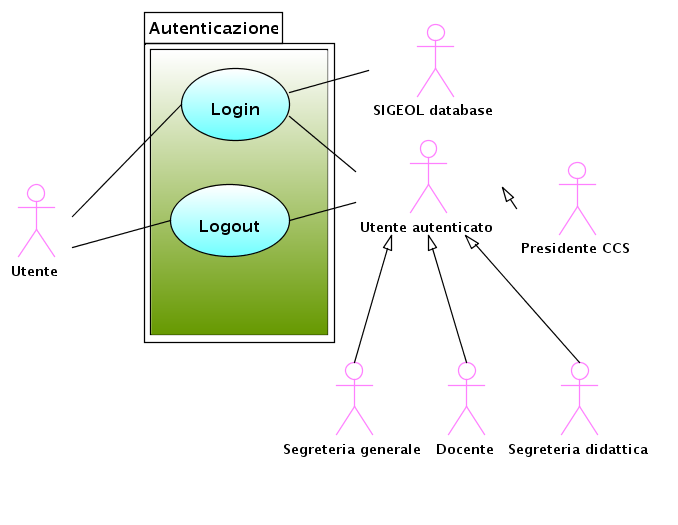
\includegraphics[scale=0.5]{UseCaseAutenticazione.png}
\end{center}
\subsubsection*{Attori coinvolti:}
\textit{utente non autenticato}, \textit{utente autenticato}, \textit{SIGEOL \underline{database}}
\subsubsection*{Scopo e descrizione sintetica:}
l'\textit{utente non autenticato} effettua l'accesso alla sua pagina personale inserendo il proprio indirizzo email nel campo 'username' e la propria password
nel campo 'password'.
L'\textit{utente autenticato} esce dal sistema premendo sul pulsante di \underline{logout}.
\subsubsection*{Pre-condizioni:}
l'\textit{utente non autenticato} accede alla pagina di \underline{login}.
\subsubsection*{Flusso base di eventi:}
\begin{itemize}
 \item l'\textit{utente non autenticato} inserisce i suoi dati di accesso e viene effettuata la verifica dei dati immessi
\item l'\textit{utente autenticato} effettua il logout 
\end{itemize}
\subsubsection*{Flussi alternativi:}
l'\textit{utente non autenticato} esce dalla pagina di \underline{login}.
\subsubsection*{Post-condizioni:}
\begin{itemize}
 \item se i dati immessi sono corretti l'\textit{utente non autenticato} risulta {autenticato} e viene indirizzato alla propria pagina personale
 \item se i dati immessi sono errati l'\textit{utente non autenticato} viene indirizzato alla pagina di \underline{login} e viene visualizzato un messaggio di errore. 
\item l'\textit{utente autenticato} diventa \textit{utente non autenticato}
\end{itemize}

\subsection{Use case Gestione notifiche}
\begin{center} 
 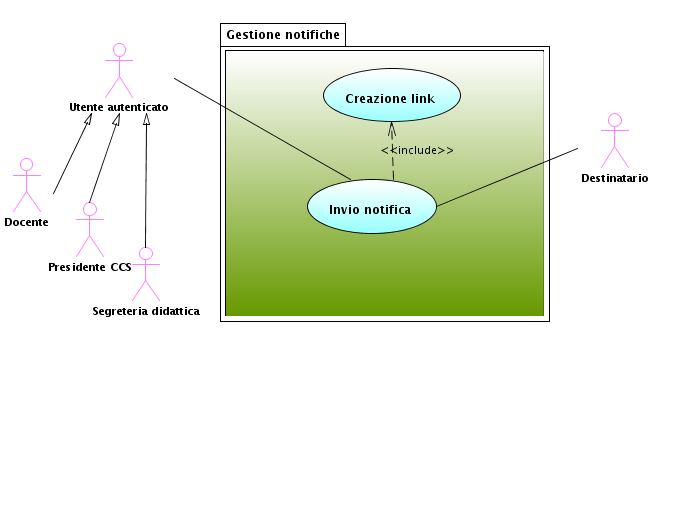
\includegraphics[scale=0.5]{UseCaseGestioneNotifiche.png} 
\end{center}
\subsubsection*{Attori coinvolti:}
\textit{segreteria generale}, \textit{segreteria didattica}, \textit{presidente CCS}, \textit{docente}
\subsubsection*{Scopo e descrizione sintetica:}
\textit{segreteria generale}, \textit{segreteria didattica}, \textit{presidente CCS}, \textit{docente} inviano una notifica o invitano un'altro utente ad entrare nel sistema. Il tipo di notifica varia in base alla funzione ad essa associata.
\subsubsection*{Pre-condizioni:}
\textit{segreteria generale}, \textit{segreteria didattica}, \textit{presidente CCS}, \textit{docente} si trovano in una delle pagine relative alla gestione dati.
\begin{itemize}
 \item \textit{segreteria generale}, \textit{segreteria didattica}, \textit{presidente CCS} scelgono di invitare nel sistema un utente
\item \textit{segreteria generale}, \textit{segreteria didattica}, \textit{presidente CCS} scelgono di inviare una notifica ad un utente
\item  \textit{segreteria generale}, \textit{segreteria didattica}, \textit{presidente CCS}, \textit{docente} ricevono un'invito o una notifica
\end{itemize}

\begin{itemize}
 \item \textit{segreteria generale}, \textit{segreteria didattica}, \textit{presidente CCS} invitano nel sistema un utente
\begin{enumerate}
 \item generazione del \underline{link} di invito
\item invio dell'invito
\end{enumerate}
\item \textit{segreteria generale}, \textit{segreteria didattica}, \textit{presidente CCS} scelgono di inviare una notifica ad un utente
\begin{enumerate}
 \item invio della notifica
 \item segnalazione della notifica nella pagina personale del destinatario
\end{enumerate}
\end{itemize}
\subsubsection*{Flussi alternativi:}
\begin{itemize}
 \item \textit{segreteria generale}, \textit{segreteria didattica}, \textit{presidente CCS} annullano l'invito
\item  \textit{segreteria generale}, \textit{segreteria didattica}, \textit{presidente CCS}, \textit{docente} annullano l'invio della notifica
\end{itemize}
\subsubsection*{Post-condizioni:}
\begin{enumerate}
 \item l'invito arriva alla casella email del destinatario
 \item la notifica viene segnalata nella pagina personale del destinatario e/o arriva alla casella email del destinatario
\end{enumerate}

\subsection{Use case Gestione facoltà}
\begin{center} 
 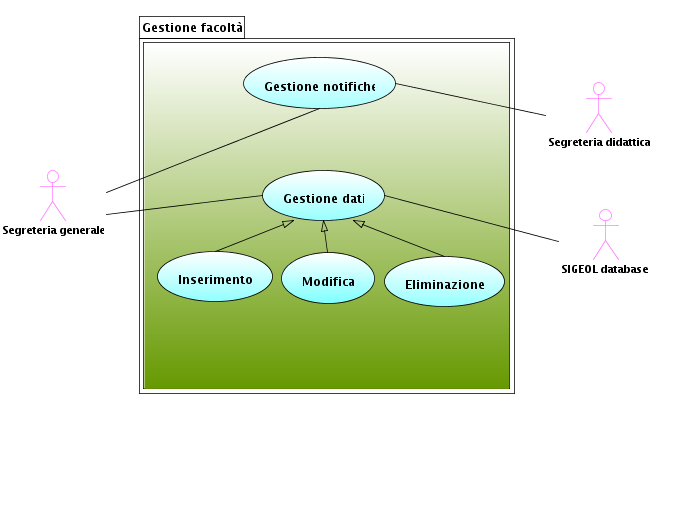
\includegraphics[scale=0.5]{UseCaseGestioneFacolta.png}
 % UseCaseGestioneFacolta.png: 801x496 pixel, 72dpi, 28.26x17.50 cm, bb=0 0 801 496
\end{center}
\subsubsection*{Attori coinvolti:}
\textit{segreteria generale}, \textit{SIGEOL \underline{database}}
\subsubsection*{Scopo e descrizione sintetica:}
la \textit{segreteria generale} inserisce, modifica ed elimina i dati relativi alle facoltà universitarie
\subsubsection*{Pre-condizioni:}
la \textit{segreteria generale} accede alla pagina della gestione facoltà
\subsubsection*{Flusso base di eventi:}
\begin{itemize}
 \item la \textit{segreteria generale} inserisce una nuova facoltà
 \item la \textit{segreteria generale} modifica i dati di una facoltà precedentemente inserita
 \item la \textit{segreteria generale} elimina una facoltà
\end{itemize}
\subsubsection*{Flussi alternativi:}
\begin{enumerate} 
 \item la \textit{segreteria generale} esce dalla pagina
\end{enumerate}
\subsubsection*{Post-condizioni:}
Le modifiche relative alle facoltà vengono inserite nel \textit{SIGEOL \underline{database}}

\subsection{Use case Gestione corsi di laurea}
\begin{center} 
 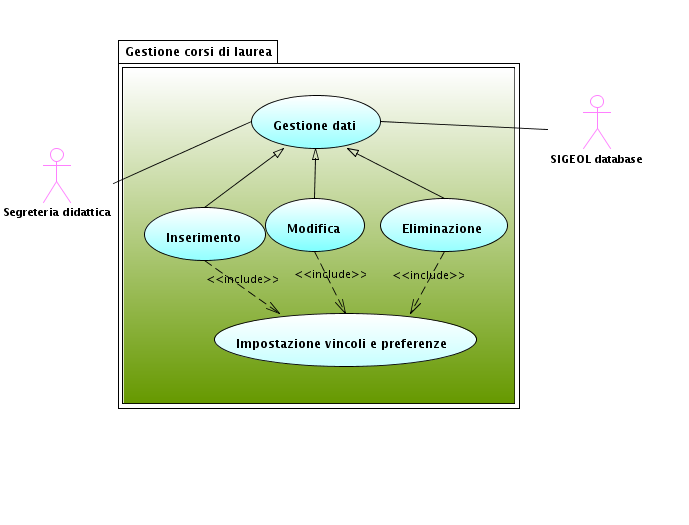
\includegraphics[scale=0.5]{UseCaseGestioneCorsiLaurea.png}
\end{center}
\subsubsection*{Attori coinvolti:}
\textit{segreteria didattica}, \textit{SIGEOL \underline{database}}
\subsubsection*{Scopo e descrizione sintetica:}
la \textit{segreteria didattica} inserisce, modifica ed elimina i corsi di laurea e i dati ad essi appartenenti
\subsubsection*{Pre-condizioni:}
la \textit{segreteria didattica} accede alla pagina della gestione corsi di laurea
\subsubsection*{Flusso base di eventi:}
\begin{enumerate}
 \item \textit{segreteria didattica} inserisce un nuovo corso di laurea
 \item \textit{segreteria didattica} modifica i dati di un corso di laurea precedentemente inserito
 \item \textit{segreteria didattica} elimina una corso di laurea già esistente
\end{enumerate}
\subsubsection*{Flussi alternativi:}
\begin{enumerate} 
\item \textit{segreteria didattica} esce dalla pagina
\end{enumerate}
\subsubsection*{Post-condizioni:}
le modifiche relative ai corsi vengono inserite nel \textit{SIGEOL \underline{database}}

\subsection{Use case Gestione corsi}
\begin{center} 
 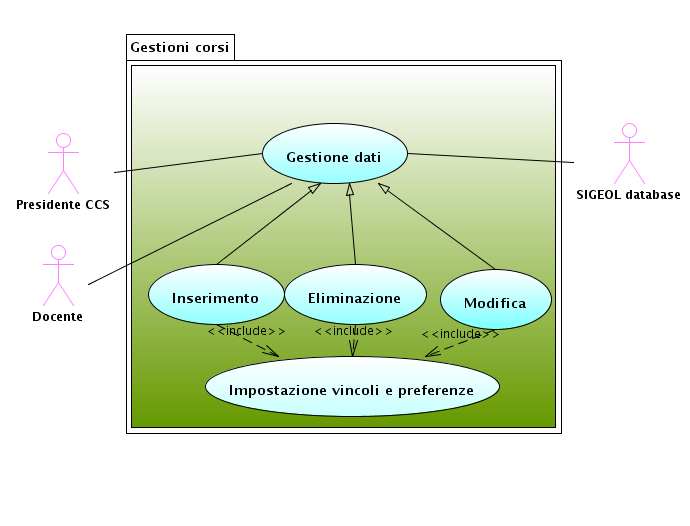
\includegraphics[scale=0.5]{UseCaseGestioneCorsi.png}
\end{center}
\subsubsection*{Attori coinvolti:}
\textit{presidente CCS}, \textit{docente},\textit{SIGEOL \underline{database}}
\subsubsection*{Scopo e descrizione sintetica:}
\textit{presidente CCS} e \textit{docente} inseriscono, modificano ed eliminano i corsi e i dati ad essi appartenenti
\subsubsection*{Pre-condizioni:}
\textit{segreteria didattica} e il \textit{presidente CCS} accedono alla pagina della gestione corsi
\subsubsection*{Flusso base di eventi:}
\begin{enumerate}
 \item \textit{segreteria didattica} e il \textit{presidente CCS} inseriscono un nuovo corso 
 \item \textit{segreteria didattica} e il \textit{presidente CCS} modificano i dati di un corso precedentemente inserito
 \item \textit{segreteria didattica} e il \textit{presidente CCS} eliminano una corso già esistente
\end{enumerate}
\subsubsection*{Flussi alternativi:}
\begin{enumerate} 
\item \textit{segreteria didattica} e il \textit{presidente CCS} escono dalla pagina
\item \textit{segreteria didattica} e il \textit{presidente CCS} inviano una notifica ad un determinato \textit{docente} a causa della sua mancata presenza nel \textit{SIGEOL \underline{database}} e quindi al momento non può essere associato al corso
\end{enumerate}
\subsubsection*{Post-condizioni:}
le modifiche relative ai corsi vengono inserite nel \textit{SIGEOL \underline{database}} e le notifiche (se effettuate) vengono correttamente 
inviate

\subsection{Use case Gestione aule}
\subsubsection*{Attori coinvolti:}
\textit{segreteria didattica}, \textit{presidente CCS}, \textit{SIGEOL \underline{database}}
\subsubsection*{Scopo e descrizione sintetica:}
la \textit{segreteria didattica} e il \textit{presidente CCS} inseriscono, modificano ed eliminano le aule e i dati ad esse appartenenti.
\subsubsection*{Pre-condizioni:}
\textit{segreteria didattica} e il \textit{presidente CCS} accedono alla pagina della gestione aule
\subsubsection*{Flusso base di eventi:}
\begin{enumerate}
 \item \textit{segreteria didattica} e il \textit{presidente CCS} inseriscono una nuova aula
 \item \textit{segreteria didattica} e il \textit{presidente CCS} modificano i dati di un'aula precedentemente inserita
 \item \textit{segreteria didattica} e il \textit{presidente CCS} eliminano un'aula già esistente
\end{enumerate}
\subsubsection*{Flussi alternativi:}
\begin{enumerate} 
\item \textit{segreteria didattica} e il \textit{presidente CCS} escono dalla pagina
\end{enumerate}
\subsubsection*{Post-condizioni:}
le modifiche relative alle aule vengono inserite nel \textit{SIGEOL \underline{database}}
\subsection{Use case Gestione docenti}
\begin{center} 
 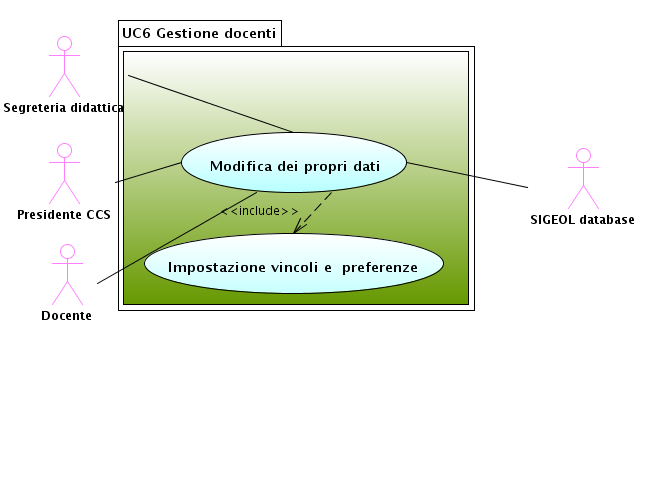
\includegraphics[scale=0.5]{UseCaseGestioneDocenti.png}
\end{center}
\subsubsection*{Attori coinvolti:}
\textit{docente}, \textit{SIGEOL \underline{database}}
\subsubsection*{Scopo e descrizione sintetica:}
il \textit{docente} modifica i propri dati personale e le proprie preferenze
\subsubsection*{Pre-condizioni:}
\textit{docente} è nella propria pagina personale
\subsubsection*{Flusso base di eventi:}
\begin{enumerate}
 \item \textit{docente} modifica i suoi dati 
 \item \textit{docente} inserisce e modifica le sue preferenze
\end{enumerate}
\subsubsection*{Flussi alternativi:}
\textit{docente} esce dalla sua pagina personale
\subsubsection*{Post-condizioni:}
le modifiche apportate vengono inserite nel \textit{SIGEOL \underline{database}}
\subsection{Use case Gestione schema d'orario}
\begin{center} 
 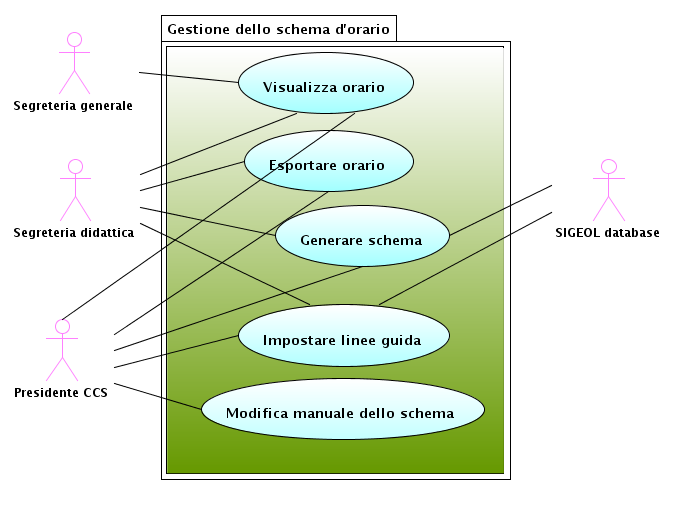
\includegraphics[scale=0.5]{UseCaseGestioneSchemaOrario.png}
\end{center}
\subsubsection*{Attori coinvolti:}
\textit{segreteria didattica}, \textit{presidente CCS}, \textit{SIGEOL \underline{database}}
\subsubsection*{Scopo e descrizione sintetica:}
\textit{segreteria didattica}, \textit{presidente CCS} possono generare, esportare e modificare lo schema d'orario
\subsubsection*{Pre-condizioni:}
\textit{segreteria didattica}, \textit{presidente CCS} accedono alla pagina della gestione dello schema d'orario.
\subsubsection*{Flusso base di eventi:}
\begin{enumerate} 
 \item \textit{segreteria didattica}, \textit{presidente CCS} generano lo schema d'orario
 \item \textit{segreteria didattica}, \textit{presidente CCS} modificano lo schema d'orario
 \item \textit{segreteria didattica}, \textit{presidente CCS} esportano lo schema dell'orario.
\end{enumerate}
\subsubsection*{Flussi alternativi:}
 \textit{segreteria didattica}, \textit{presidente CCS} escono dalla pagina di gestione dello schema d'orario.
\subsubsection*{Post-condizioni:}
\begin{enumerate}
 \item l'orario viene esportato nel formato scelto.
 \item l'orario viene salvato nel \textit{SIGEOL \underline{database}}
\end{enumerate}  

\subsection{Use case Gestione consultazione}
\begin{center} 
 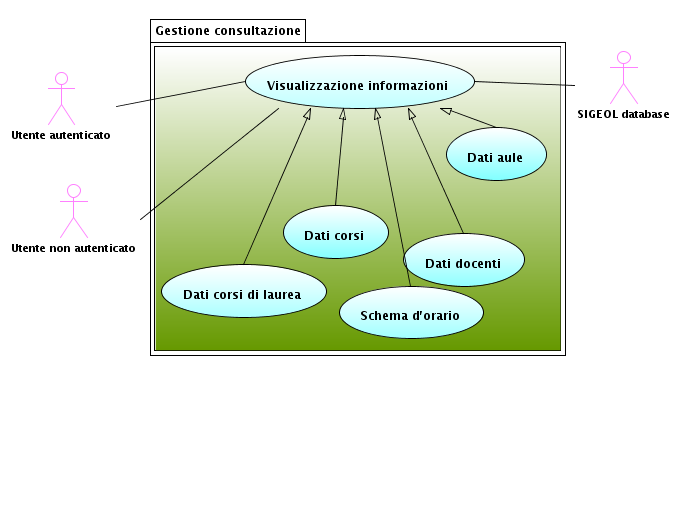
\includegraphics[scale=0.5]{UseCaseGestioneConsultazione.png}
\end{center}
\subsubsection*{Attori coinvolti:}
\textit{utente autenticato}, \textit{utente non autenticato}
\subsubsection*{Scopo e descrizione sintetica:}
\textit{utente autenticato}, \textit{utente non autenticato} possono visualizzare le informazioni relative ai corsi di laurea, corsi di lezione, docenti, aule e schema d'orario
\subsubsection*{Pre-condizioni:}
\textit{utente autenticato}, \textit{utente non autenticato} accedono alla pagina della gestione consultazioni
\subsubsection*{Flusso base di eventi:}
\textit{utente autenticato}, \textit{utente non autenticato} visualizzano le informazioni relative ai corsi di laurea, corsi di lezione, docenti, aule e schema d'orario
\subsubsection*{Flussi alternativi:}
 \textit{utente autenticato}, \textit{utente non autenticato} escono dalla pagina di gestione consultazione

\subsection{Use case Gestione backup}
\begin{center} 
 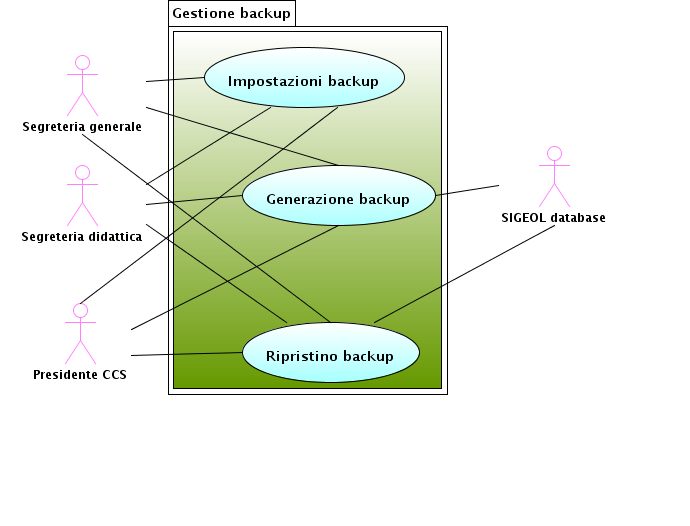
\includegraphics[scale=0.5]{UseCaseGestioneBackup.png}
\end{center}
\subsubsection*{Attori coinvolti:}
\textit{segreteria generale}, \textit{segreteria didattica}, \textit{presidente CCS}, \textit{SIGEOL \underline{database}}
\subsubsection*{Scopo e descrizione sintetica:}
\textit{segreteria generale}, \textit{segreteria didattica}, \textit{presidente CCS} impostare le preferenze per la generazione dei \underline{backup}, generano il \underline{backup} e ripristinano precedenti \underline{backup} del \textit{SIGEOL \underline{database}}
\subsubsection*{Pre-condizioni:}
\textit{segreteria generale}, \textit{segreteria didattica}, \textit{presidente CCS} sono nella pagina della gestione dei \underline{backup}
\subsubsection*{Flusso base di eventi:}
\begin{itemize}
 \item \textit{segreteria generale}, \textit{segreteria didattica}, \textit{presidente CCS} modificano le impostazioni di \underline{backup}
 \item \textit{segreteria generale}, \textit{segreteria didattica}, \textit{presidente CCS} generano un \underline{backup}
 \item \textit{segreteria generale}, \textit{segreteria didattica}, \textit{presidente CCS} ripristinano un \underline{backup} già esistente
\end{itemize}
\subsubsection*{Flussi alternativi:}
\textit{segreteria generale}, \textit{segreteria didattica}, \textit{presidente CCS} escono dalla pagina della gestione dei \underline{backup}
\subsubsection*{Post-condizioni:}
\begin{itemize}
\item le impostazioni vengono salvate
\item il \underline{backup} viene generato
\item viene ripristinato il \textit{SIGEOL \underline{database}} con un \underline{backup} precedente
\end{itemize}

\modifiche
\end{document}
